\section{Квазипериодическое движение \texorpdfstring{($\S 30$)}{Lg}
}
Образом стационарного движения служит точка, образом периодического -- замкнутая траектория (предельная точка или предельный цикл).  
\subsection{Мультипликатор}

При $\R > \R_{\text{кр}}$ возможны различные устойчивые режимы. Роль невозмущенного движения играет периодическое $\vc{v}_0(r, t)$. Уравнение движения -- $\vc{v} = \vc{v}_0 + \vc{v}_2$, где $\vc{v}_2$ -- малая поправка. 

Но $\vc{v}_2$ функция не только координат, но и времени, причем по времени эти коэффициенты представляют периодические функции с периодом $T_1 = 2 \pi / \omega_1$. Решение такого уравнения ищется в виде:
\begin{equation}
    \vc{v}_2 = \Pi(\vc{r}, t) e^{-i\omega t},
\end{equation}
где $\Pi(\vc{r}, t)$ -- периодическая функция времени. Неустойчивость возникает при появлении частоты $\omega = \omega_2 + i \gamma_2$, c $\Im = \gamma_2 > 0$, а $\Re = \omega_2$ определяет новую частоту. 

За период $T_1$ возмущение меняется $\mu \equiv e^{-i\omega T_1}$ раз. Этот множитель -- \textbf{мультипликатор} периодического движения, характеристика усиления или  затухания возмущений этого движения. 

Потеря устойчивости происходит при числе $\R_{\text{кр2}}$, при котором один или более мультипликаторов по модулю становятся равными 1. Ввиду вещественности уравнений мультипликаторы проходят окружность или парами, или в  точках $\pm 1$. Потеря устойчивости периодическим движением сопровождается определенной качественной перестройкой поведения траекторий в пространстве состояний в окрестности ставшего неустойчивым предельного цикла -- локальной \textbf{бифуркацией}\footnote{
    Характер бифуркации в значительной степени определяется именно тем, в каких точках единичной окружности мультипликаторы её пересекают.
}. 

%%%%%%%%%%%%%%%%%%%%%%%%%%%%%%%%%%%%%%%%%%%%%%%%%%%%%%%%%%%%%%%%%%%%%%%%

\subsection{<<Рождение>> двумерного тора}

\begin{wrapfigure}{r}{0.3\linewidth}
    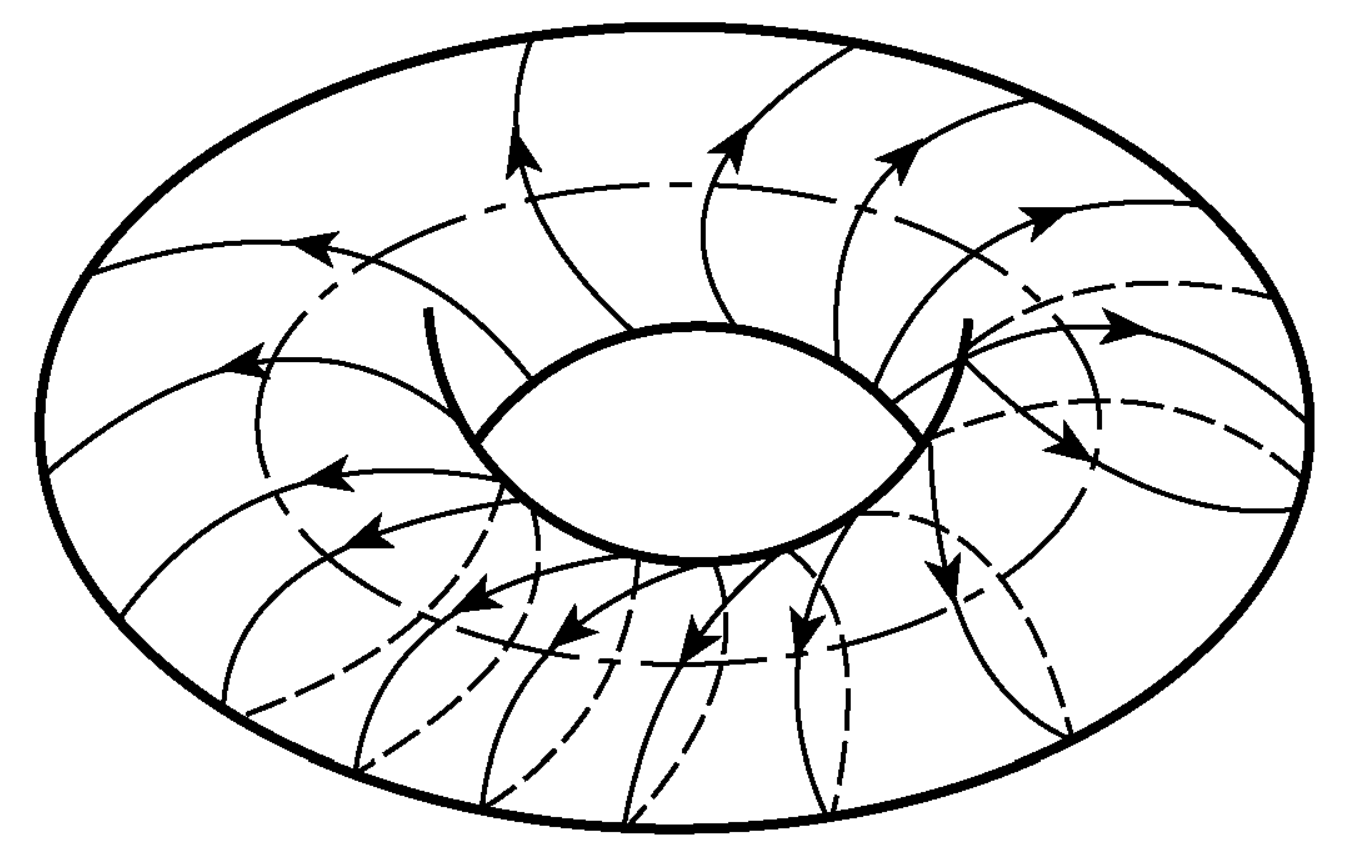
\includegraphics[width=\linewidth]{img/tor.png}
\end{wrapfigure}

Рассмотрим бифуркацию пересечения единичной окружности мультипликаторов вида $\mu = \exp{\left(\pm 2 \pi \alpha i\right)}$, где $\alpha \in \mathbb{R} \setminus \mathbb{Q}$. Это приводит к появлению вторичного течения с новой независимой частотой $\omega_2 = \alpha \omega_1$, т.е. в результате возникает некоторое \textbf{квазипериодическое движение}, характеризующееся двумя несоизмеримыми частотами. Геометрическим образом этого движения в пространстве состояний служит траектория в виде незамкнутой намотки на двумерном торе, причём ставший неустойчивым предельный цикл служит {образующей} тора: $\omega_1$ -- вращение по образующей, $\omega_2$ - вращение на торе. 
Получается перешли от движения с одной степенью свободы к движению с двумя. 

Рассмотрим \textbf{гипотетическую} картину усложнения течения, возникшего в результате такой бифуркации, при дальнейшем увеличении $\R$, $\R > \R_{\text{кр2}}$. Естественно было бы пред
положить что при последующем увеличении $\R$ будут последовательно появляться все новые периоды. Это означает потерю устойчивости двумерным о тором с возникновением в его окрестности трехмерного тора, затем в результате очередной бифуркации ему на смену придет 4-мерный тор и т.д. Интервалы между числами Рейнольдса соответствующими появлению новых частот , быстро падают , а появляющиеся движения имеют все меньшие масштабы. Таким образом движение быстро приобретает сложный характер --- турбулентный. 

Такая \textbf{гипотетически} возможная модель перехода к турбулентности былы предложена \textit{Л.Д. Ландау (1944)} и, независимо, \textit{Э. Хопфом (1948)}.

%%%%%%%%%%%%%%%%%%%%%%%%%%%%%%%%%%%%%%%%%%%%%%%%%%%%%%%%%%%%%%%%%%%%%%%%

\subsection{Cценарий Ландау-Хопфа}

Напишем общий вид функции $\vc{v}(\vc{r}, t)$, зависимость которой от времени определяется некоторым $N$ различных частот. Искомая функция может быть представлена в виде ряда
\begin{equation}
    \vc{v}(\vc{r}, t) = \sum \vc{A}_{p_1 p_2 \ldots p_N} (\vc{r}) \exp \left(-i \sum_{i=1}^{N} p_i \varphi_i \right),
\end{equation}
Все различные фазы лежат в интервале $0 \leq \varphi \leq 2 \pi$. Рассмотрим пару фаз. Пусть в некоторый момент времени $\varphi_1$ имеет значение $\alpha$. Тогда <<одинаковые>> с $\alpha$ значения фаза $\varphi_1$ будет иметь и во все моменты времени
$$
    t = \frac{\alpha - \beta_1}{\omega_1} + 2 \pi s \frac{1}{\omega}.
$$
Фаза $\varphi_2$ в эти моменты имеет значения
$$
\varphi_2 = \beta_2 + \frac{\omega_2}{\omega_1}\left(\alpha - \beta_1 + 2 \pi s\right).
$$
Но различные частоты несоизмеримы друг с другом, так что $\omega_2/\omega_1$ -- иррациональное число. Приводя каждый раз посредством вычитания должного кратного от $2\pi$ значение $\varphi_2$ к интервалу, мы получим для $\varphi_2$ значения сколь угодно близкие к любой паре наперед заданных значений. 

Таким образом в рассматриваемой модели турбулентности в течение достаточно долгого времени жидкость проходит через состояния, сколь угодно близкие к любому наперед заданному состоянию. Время возврата, однако, растет с увеличением $N$ и становится столь большим, что никакого следа периодичности не остается. 

 Стоит подчеркнуть, что рассмотренный путь возникновения турбулентности базируется на \textbf{линейных} представлениях. Фактически предполагалось, что при появлении в результате неустойчивости новых периодических решений уже имевшиеся периодические решения не только не исчезают, но и почти не меняются. В данной модели турбулентное движение есть просто суперпозиция большого числа таких не изменяющихся решений. В общем же случае характер решений изменяется. Возмущения взаимодействуют друг с другом, причём это может привести как к упрощению движения, так и к его усложнению. 

%%%%%%%%%%%%%%%%%%%%%%%%%%%%%%%%%%%%%%%%%%%%%%%%%%%%%%%%%%%%%%%%%%%%%%%%

\subsection{Синхронизация колебаний}

Рассмотрим простой случай: возмущенное решение содержит две независимые частоты. Возмущение на частоте $\omega_1$ (от $\R = \R_{\text{кр1}}$), естественно считать в окрестности числа $\R = \R_{\text{кр2}}$ более интенсивным и поэтому полагать его неизменным при относительно небольших изменениях числа $\R$ в этой окрестности. Имея это в виду для описания эволюции возмущения с частотой $\omega_2$ на фоне периодического движения частоты $\omega_1$ введем новую переменную
\begin{equation}
    a_2(t) = |a_2(t)|e^{-i\varphi_2(t)};
\end{equation}
модуль $|a_2|$ -- кратчайшее расстояние до образующей тора, а $\varphi_2$ -- его фаза. Рассмотрим поведение $a_2$ в дискретные моменты времени. За время одного периода возмущение частоты $\omega_2$ меняется в $\mu$ раз, где:
$$
\mu = |\mu| \exp \left(-2\pi i \omega_2/\omega_1\right)
$$
-- его мультипликатор. Далее рассмотрим уравнения относительно дискретной переменной числа прошедших периодов ($a_2$) $\tau$. Можем прийти к уравнению
$$
\frac{d a_2}{d \tau} = \ln \mu \cdot a_2 - \beta_2 a_2 \cdot |a_2|^2.
$$
Вещественная часть уравнения определяет стационарное значение модуля, мнимая -- уравнение для фазы:
\begin{equation}
    \label{mnim}
    \frac{d\varphi_2}{d\tau} = 2 \pi \frac{\omega_1}{\omega_2} + \Im \beta_2 \cdot |a_2|^2
\end{equation}
Согласно этому фаза $\varphi_2$ вращается с постоянной скоростью (связано с приближением). С ростом надкритичности равномерность нарушается и скорость вращения по тору становится функцией $\varphi_2$. Чтобы это учесть, добавим в \eqref{mnim} малое возмущение $\Phi$. Далее аппроксимируем иррациональное отношение $\omega_2/\omega_1$ рациональной дробью $m_2/m_1$. Так получим уравнение:
\begin{equation}
\label{30.8}
    \frac{1}{m_1} \frac{d \varphi}{d\bar \tau} \sim \Im \beta_2 \cdot |a_2|^2 + \Phi.
\end{equation}

В общем случае уравнение \eqref{30.8} имеет стационарные решение $\varphi_2 = \varphi_2^{\text{0}}$, но также мы получаем, что \textbf{на торе существует предельный цикл -- траектория через $m_1$ оборотов замыкается.}

Рождение устойчивого предельного цикла на торе означает \textbf{синхронизацию} колебаний -- исчезновение квазипериодического и установление нового режима. Это явление препятствует возникновению режима, представляющего собой суперпозицию движений с большим числом несоизмеримых частот. В этом смысле можно сказать, что \textbf{вероятность реального осуществления сценария Ландау-Хопфа мала.}

\textbf{Но, например}, в \cite{LH1} рассматриваются системы поведение которых близко к описанному сценарию.

